\chapter{Summary}\label{sec:summary}

This thesis has presented two analyses of the proton-proton collision data collected by ATLAS during the LHC Run~2.
This data was produced in proton-proton collisions at center-of-mass energy of 13 TeV at the LHC.
The full dataset was collected by the ATLAS experiment between the years 2015 and 2018 and corresponds to an integrated luminosity of 139 fb$^{-1}$.
The focus of both analyses is on collision events containing two charged leptons in the final state.
The clean experimental signature and fully reconstructable nature of these events make them a particularly appealing window into the nature of fundamental particles.


% ======== Hmumu ======== 
The search for the Higgs decay to two muons investigates events with dimuon pairs in the final state.
Central to this study is the Yukawa coupling, $H\mu\mu$, that is thought to provide the muon with its mass.
This coupling is interesting from two perspectives.
First, as the source of the muon's mass, the coupling differentiates the muon from the lighter electron and heavier tau.
It is a fundamental characteristic of the muon.
Different Yukawa couplings have only been observed with heavier third-generation fermions.
Second, studying the coupling is part of a broader project to measure the properties of the Higgs boson.

Presently no observation of the coupling has reached a significance of $3\sigma$.
The significance of the \hmm signal strength measured by ATLAS using Run~2 data is 2$\sigma$, which exceeds the sensitivity predicted at the start of the run by over 30\%. 
This improvement is primarily due to the highly optimized use of multivariate analysis categorization.
Future operation of the LHC promises to enable more detailed study.
The upcoming LHC Run~3 will likely provide enough collision data to allow an observation at the level of ``evidence'' ($\approx3\sigma$ significance).
In the coming decades, planned luminosity upgrades to the LHC should allow for a measurement to exceed the level of $7\sigma$ significance.
These precise measurements will form an interesting test of the predictions of the Standard Model.

% Future improvements to the analysis
The analysis of the complete Run~2 dataset with respect to \hmm is part of a series of related analyses that extends to the past, and is expected to continue in the future.
The strategies adopted in each iteration reflect both the amount of data available to analyze and the lessons learned from previous work.
Future iterations may expand their focus to include bbH production, the bottom quark analog to ttH.
These studies may also reduce their reliance on simulation in order to isolate their results from theoretical and experimental uncertainties.
Precautions should be taken in the broader \hmm analysis to train the multivariate discriminant in the same phase space in which it will be used, as was done in the VH analysis.
% Further consideration as to the advantage in estimated sensitivity from the proliferation of ever smaller categories compared to the statistical challenge these raise.
A blinding strategy, similar to that used in the VH analysis, could be adopted more broadly. 
In this case the parameters defining the analysis categorization and background modeling are frozen before observing the measured data.
This helps avoid a major source of bias.

A major focus of this thesis has been on the VH production mechanism in conjunction with the \hmm process.
This is the first investigation of the previously unexplored multi-leptonic phase spaces of \vhllmm.
Newly introduced model-independent limits are set in this phase space using an inclusive categorization for VH-like events.
Modern statistical techniques related to the multivariate categorization, including the use of cross-validation, result in robust exclusive categories with reduced bias.
Small excesses of events are observed in the VH signal regions.
These results were published on January 2021 in Physics Letters B \cite{atlasHmm}.
After the publication of these results, the CMS Collaboration released their observation showing a similar excess in VH-like events \cite{cmsHmm}.
New limits are set on the Higgs production in these inclusive categories.

% Future improvements to the analysis
Future iterations of the VH analysis may consider the quark decays of the vector bosons, resulting in final state jets.
Another promising inclusion is the $Z\to\nu\nu$ decay mode identified by \met signatures.
These approaches were found to be insensitive at present when compared to considering these events together with ggH and VBF events.
Improvements in \met and jet reconstruction and resolution could make such these challenging VH categories competitive.
% A similar situation exists for ZH events where the \Z decays to neutrinos.

% ========  CI   ======== 
The search for new physics with non-resonant features in the high-mass tail of the dilepton invariant-mass spectra complements the search for \hmm.
The strategy taken in this analysis offers a stark departure from previous studies.
In addition to using a background estimate derived from data, the statistical treatment of the observation is strengthen by the use of frequentist methods.
The analysis exchanged theoretical uncertainties for experimental and statistical uncertainties.
Additionally, a new method for estimating the sensitivity of the result to mis-modeling effects was developed and introduced. 
These improvements parted with the tradition of ATLAS, and it took a nearly year of detailed investigation for them to be accepted by the collaboration.
These results were published on November 2020 in the Journal of High Energy Physics\cite{ciAaron}.
The publication of this result paves the way for future analyses based on these methods.
\footnote{Currently a study of the clockwork mechanism a search for large extra dimensions have moved in this direction.}

% \footnote{In some cases, resistance was particularly emotional as evinced by the comment: ``in the unlikely event that you re being serious here, let me just inject that this paper would likely top the charts of the most embarrassing estimates of SM background that this collaboration has ever produced.''}

\begin{figure}[h!]
\centering
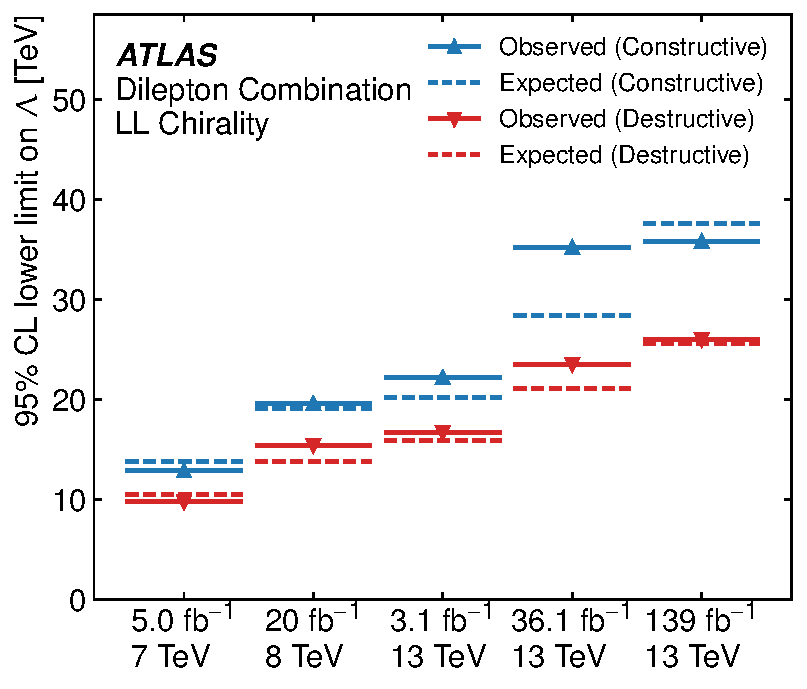
\includegraphics[width=0.70\textwidth]{figures/ci/results/figaux_05.pdf}
\caption{Comparison of the $\ell\ell$ constructive (blue) and destructive (red) LL chirality limits with previous ATLAS results. For results with Bayesian limits, the $\Lambda^{-4}$ prior is used. ($\sqrt{s}=13$~TeV 36.1 fb$^{-1}$ result: \cite{EXOT-2016-05}, $\sqrt{s}=13$~TeV 3.1 fb$^{-1}$ result: \cite{EXOT-2015-07}, $\sqrt{s}=8$~TeV 20 fb$^{-1}$ result: \cite{EXOT-2013-19}, $\sqrt{s}=7$~TeV 5.0 fb$^{-1}$ result: \cite{EXOT-2012-17}.)}
\label{fig:ciAtlasHistoricalLimits}
\end{figure}

The search for new physics with non-resonant features takes a different approach than the \hmm search.
Despite the inclusive results, the target of \hmm search is the particular dimuon resonant signature produced by specific mechanisms in the Standard Model.
The model-independent results play an auxiliary role.
In contrast, the analysis of the high-mass dilepton spectra searches for unexpected deviations regardless of their source.
The key result are the limits on the \xsbr in each signal region, which are agnostic as to the production mechanism.
These limits are the first of their kind.
They are provided along with the necessary information to interpret them in terms of new hypotheses that predict non-resonant event production in the analysis signal regions.

More conventional limits are set on the energy scale, \lam, of contact interactions.
Such interactions are of particular interest because they enable probes of enormous energy scales that are not directly accessible at the LHC. 
Contact interactions are intriguing as the signature of composite fermions.
The exclusion of contact interactions necessarily limits fermion binding energy if they are composite.
It is for these reasons that contact interactions have held the interest of particle physicists for so long, as illustrated in Figure \ref{fig:ciAtlasHistoricalLimits}.
Here the evolution of ATLAS results is shown using various collision energies and luminosities.
The results are arranged chronologically based on their publication.
The steady progression of the search sensitivity can be seen over time by the evolution of the expected limits; the left-left chirality results produced by this analysis appear in the right-most bin.
These eventually reach the staggering energy scales of 35.8~TeV and 28.8~TeV for constructive and destructive CI respectively.

% Future improvements to the analysis
It is somewhat subjective to predict the future performance of non-resonant searches.
Unlike the search for \hmm, where the result is limited statistically by the availability of data, this search is carried out in the tail of the invariant-mass spectra.
The extent of the tail is influenced more by the center-of-mass energy than event multiplicity.
Nevertheless a simple extrapolation predicts that, with $\sqrt{s}=13$~TeV collisions and the predicted integrated luminosity of 300 \fb of Run~3, the sensitivity may reach 43~TeV and 29~TeV for constructive and destructive CI respectively.
These improvements would be enhanced by the anticipated arrival of $\sqrt{s}=14$~TeV collisions.

The model-dependant results for CI are sensitive to systematic uncertainties on the expected event multiplicity for a given value of \lam.
These uncertainties, especially those with experimental origins, can be reduced by a better understanding of the performance of the ATLAS detector.

% ============= Wrap up ===============

 \threestars


The strategy of the \hmm and non-resonant searches represent very different approaches with a similar goal: to advance our knowledge of Nature at its most fundamental scales.
The \hmm analysis focuses on a specific prediction, and is designed with a singular vision of searching a narrow phase space for a well defined signal predicted by the Standard Model.
This approach benefits from its concentrated focus and suffers from its lack of generality.
The non-resonant analysis eschews a signal model and searches for unexpected phenomena beyond the predictions of the Standard Model, only to interpret the results in terms of a broad description of contact interactions.
This approach benefits from its unrestricted scope and suffers from its lack of optimization to a specific signal.
These strategies complement each other, making up for the others shortcomings, and together comprise the armamentarium of methods used to study the Universe.
